\documentclass[preprint]{elsarticle}
\biboptions{round, numbers}
\usepackage[latin1]{inputenc}
%\usepackage[T1]{fontenc}
%\usepackage{textcomp}
\usepackage{graphicx}
\usepackage{color}
%\usepackage{setspace}
\usepackage{url}
\usepackage[english]{babel}

\begin{document}

\begin{frontmatter}

%%%%%%%%%%%%%%%%%%%%%%%%%%%%%%%   TITLE   %%%%%%%%%%%%%%%%%%%%%%%%%%%%%%%

\title{Corporate Security Solutions for BYOD.\\ A Novel User-Centric and Self-Adaptive System}

%%%%%%%%%%%%%%%%%%%%%%%%%%%%%%%   AUTHORS   %%%%%%%%%%%%%%%%%%%%%%%%%%%%%%%

\author{P. de las Cuevas, A.M. Mora, J.J. Merelo}
\ead{\{paloma, amorag, jmerelo\}@geneura.ugr.es}
\address{Departamento de Arquitectura y Tecnolog�a de Computadores.\\ ETSIIT - CITIC. University of Granada, Spain}
%\author{A. M. Mora}
%\ead{amorag@geneura.ugr.es}
%\address{Departamento de Arquitectura y Tecnolog�a de Computadores. Escuela T�cnica Superior de Ingenier�as Inform�tica y de Telecomunicaci�n. CITIC. University of Granada, Spain}

%\maketitle

%
%%%%%%%%%%%%%%%%%%%%%%%%%%%%%%%%%   ABSTRACT   %%%%%%%%%%%%%%%%%%%%%%%%%%%%%%%%%
%
\begin{abstract} 
Enterprises, and their Chief Security Officers (CSOs) particularly, want to be sure that their Security Policies are complied. This goal turned hard to achieve since employees are able to use their own devices (laptops, smartphones, and tablets) at work, or at home but for work purposes. As this is part of the Bring Your Own Device (BYOD) philosophy and is being adopted by many companies everyday, a number of solutions have arisen in order to adapt it securely. In this paper, a novel system to deal with this situation is introduced, named  MUSES (Multiplatform Usable Endpoint Security). It is a system able to cope with security issues regarding the enterprise security policies, but as a user-centric tool, which considers system user's behaviour in order to adapt, improve, or even increase the defined set of security rules. MUSES applies machine learning and computational intelligence techniques in order to do this, and also would be able to predict future security incidences produced by these users.
This system, still in development, is compared with the most relevant solutions offered by other companies to deal with the same issues as MUSES, remarking the advantages that our system will offer with respect to them.
\end{abstract}

%
%%%%%%%%%%%%%%%%%%%%%%%%%%%%%%%%%   KEYWORDS   %%%%%%%%%%%%%%%%%%%%%%%%%%%%%%%%%
%
\begin{keyword}
Corporate mobile security \sep End-to-end security solutions \sep User-centric systems \sep Self-adaptation \sep Multiplatform \sep Security Policies \sep Data security and data privacy \sep BYOD
\end{keyword}

\end{frontmatter}


%-------------------------------------------------------------------------------
%%%%%%%%%%%%%%%%%%%%%%%%%%%%%%%   INTRODUCTION   %%%%%%%%%%%%%%%%%%%%%%%%%%%%%%%
%-------------------------------------------------------------------------------

\section{Introduction}
\label{sec:intro}

The way on how data has been stored and accessed in the companies has completely changed along the years. The use of owned servers being accessed by desktop PCs (and maybe laptops) from inside the company facilities has been transformed into the distribution of these data among a number of machines, even not all belonging to the company, and working over the famous Cloud Computing environment. Besides, being stored in the cloud or not, data are being consulted and modified through a wide amount of devices, some of them owned by the company's users. This is the so-called Bring Your Own Device (BYOD) philosophy. It is becoming highly successful due to the impact that portable devices (such as smartphones and tablets) are having in the market.
Data security and privacy are key factors for a company, thus, to protect them, it is usual to define Organisational Security Policies. Their definition is nowadays a very difficult problem, since the BYOD tendency means that several factors must be considered \cite{Opp_Security11}, most of them previously ignored or non considered in security systems, for instance the current mixture between personal and professional information in these devices (the user could navigate inside social networks where there could be friends and also company partners or clients).

In this scenario several solutions have arisen in order to manage the corporate security. Some solutions are focused only in smartphones, while others are thought for laptops; also some are implemented for a certain platform, but others consider multiplatform. However most of them try to be non-intrusive (regarding the users' personal data), friendly and easy to use. 

Moreover, it has been demonstrated that people are the main hazard regarding the company security \cite{Adams_Users05}, so in this situation, some monitorization and security-aimed applications are arising, aiming to cope with the concept of seamless working experience on different devices. 
This concept is a methodology of work which allows users to start/continue a working session over multiple devices and locations without any significant loss of data. This new situation has a big impact from the point of view of the security \cite{Schu_SecPatterns05}, since the company's data borders have changed in the last years so now the users can access significant data from outside the enterprise, and possibly through a non absolutely secure channel.

Thus, this work introduces a novel (still in development) system named MUSES, from Multiplatform Usable Endpoint Security, which is a device-independent end-to end user-centric tool, based in a set of security rules defined as specifications of the Corporate Security Policies, but with the ability of `learning' from the user's past behaviour and adapt, even inferring new ones, the set of rules in order to deal with potential future security incidents due to the user's. Then the system will react, in a non-intrusive way, to the potentially dangerous sequence of actions (events) that he or she is conducting at any time.

To this end MUSES will analyse the users' behaviour by means of Data Mining (DM) techniques \cite{DataMining_Lee01} and Machine Learning (ML) methods \cite{MachineLearning_Bishop06}, extracting a set of patterns which will be later processed by means of Computational Intelligence (CI) algorithms, namely Evolutionary Computation methods \cite{EAs_Back96,GP_Koza92}.

MUSES will include some important modules in the loop, such as an Event Processor, which performs an event correlation task \cite{SurveyEventCorrelation_Tiffany02}, matching occurred events with rules to deal with them and extracting threads that a Real-Time Risk and Trust Analysis Engine (RT2AE) \cite{RT2AE_SOTICS13} will process (along with other trust data and profiles), to select the best subset.

In the paper the system architecture is presented, in addition to a deep description of the soft computing methods the system will apply.

But first, this work presents a brief overview of the main existing solutions in this environment. Then a comparison between these tools and MUSES is also conducted, focusing on the advances beyond the state of the art that this novel system (being developed inside an European Project\footnote{\url{http://musesproject.eu/}} of the same name) will bring. 

The rest of the paper is organized as follows. First, some background situation about enterprise security is presented in Section \ref{sec:preliminaryconcepts}, explaining how BYOD philosophy affects it. Then, the main tools/solutions are detailed in Section \ref{sec:toolsreview}, even if they are still in development.  
Then, in Section \ref{sec:muses}, the Multiplatform Usable Endpoint Security System is presented (architecture + soft computing techniques). Its advantages and benefits in comparison with the other solutions are commented in Section \ref{sec:comparison}.
Finally, the reached conclusions are discussed in Section \ref{sec:conclusions}.


%----------------------------------------------------------------------------
%%%%%%%%%%%%%%%%%%%%%%%%%%%%%%%   BACKGROUND  %%%%%%%%%%%%%%%%%%%%%%%%%%%%%%%
%----------------------------------------------------------------------------


\section{Preliminary concepts and background about enterprise security}
\label{sec:preliminaryconcepts}

One of the tasks of a Chief Security Officer (CSO) is to elaborate an efficient set of Information Security Policies (ISPs), for controlling a certain, and already known, structure \cite{Opp_Security11}. This means that, until the appearance of BYOD, enterprises used to follow static security policies devoted to control an environment where the company assets and the devices were purchased and maintained by the company. Now that corporate networks are becoming dynamic for being adapted to this BYOD philosophy, there is an additional risk because the devices that the employees use are not always company-owned. This means that the CSOs have to find the balance between having a fast response to any user action that might cause harm (in terms of money loss because of a security incident), and trying to avoid monitoring the users in a way that is against privacy. A needed security policy, or in this case, an ISP should deal with the way of protecting a certain organization's information against a security breach. Though there are standards, such as the ISO27002 or the Security Forum's Standard of Good Practice\footnote{\url{https://www.securityforum.org}}, and many guidelines \cite{SecPol09}, an ISP should be adapted depending on the characteristics of the community/organisation that they are built for. In this sense, MUSES stands up for a self-adaptation of the security policies of a company.

On the other hand, employee-owned devices like smartphones, can be both used for personal matters at work, and for continue working outside of the workplace. As the name says, smartphones are more than simple mobile phones, and people who use them in their works have the possibility of maintaining a good balance between work and private life. For this reason, the risk of uncontrolled devices accessing to corporate assets in unsafe conditions, due to the number of new risks which are linked to smartphones \cite{gangula2013survey}, is bigger.

Normally, the enterprise network architecture was being adapted to cope with external attackers \cite{MIT05}. With the incorporation of BYOD, the threat is about corporate assets being compromised due to employees' devices with vulnerabilities \cite{android11}, or leaked because they are being accessed from a device connected through an insecure (public) network.

Thus now, more risky situations should be considered when designing a company's network architecture. In Figure \ref{fig:proposed_diagram} there is a proposal which can be used for the beginning of the study of solutions that may secure such a dynamic environment. It includes the possibility of having employee-owned mobile (smartphones and tablets) and portable (laptops) devices, and also the opportunity that the employees have of connecting these devices either from inside or outside the company premises. Moreover, company's information assets are constantly accessed under these conditions, considering that an information asset means every \textit{piece of information} that has a \textit{value} (cost depending on the risk of being lost or leaked) for the company. It can be referred to files with sensitive information, as well as confidential mails, or even to company applications.

\begin{figure}[ht]
	\begin{center}
		\includegraphics[scale=0.4]{img/proposed_diagram.eps}
		\caption{Architecture approach of an enterprise network, assuming that it has adopted the BYOD philosophy.}
	\label{fig:proposed_diagram}
	\end{center}
\end{figure}

The other issue to cope with is the elaboration of a good ISP, understandable for every user of the company, and more importantly, non-intrusive for him. A lot of researchers have studied the natural tendency of employees to comply with the ISP \cite{SecPolComp10,SecPolComp12,SecPolComp14}, reaching conclusions such as the employees compliance with the security policies increases educating/training them in information security awareness  \cite{SecPolComp09}, and decreases applying too much sanctions when a misuse or abuse occurs \cite{SecPolPenalty09}. Thus, in this paper, for each tool in Section \ref{sec:toolsreview} it is specified if the developers have taken into account the construction of ISPs, or even if they give some guidelines for building them.

This situation leads to a need of protecting the organisation's side, but also the users' side, making non-interfering easy-to-follow ISPs, and leaving them to use their devices for personal purposes while working, without putting organisation's information assets under risk. The compliance of these requirements would compose an End-to-End Security Solution (protecting both enterprise and employee), which is the motivation of the commented tools and, as presented in Section \ref{sec:muses}, is the aim of the MUSES project.


%------------------------------------------------------------------------------
%%%%%%%%%%%%%%%%%%%%%%%%%%%%%%%   TOOLS REVIEW  %%%%%%%%%%%%%%%%%%%%%%%%%%%%%%%
%------------------------------------------------------------------------------

\section{Tools for corporate mobile security}
\label{sec:toolsreview}

Many tools for companies, as well as for devices, which have adopted the BYOD have been released in the past four years. This way, and
more focused on the enterprise, there are some tools which offer the CSO ways to control the devices which enter in the system, requiring users to employ strong passwords, for instance, and also to protect the employees data by means of data encryption and data protection by having strong and secure passwords. Other tools for managing a BYOD situation add to their features guidelines for the CSOs to develop good ISPs. On the other hand, many solutions have been presented which are more focused on the device side, although they implement also the server side. Some of those tools have influenced the development of the MUSES system  itself (Section \ref{sec:muses}), which can complement them, as adds other features that go beyond the state of the art. The present section introduces the most relevant features of these products, as they can be considered related to the MUSES objectives.

% Don't completely like the intro for being too focused to MUSES.

%----------------------------------------------------------------------------

\subsection{IBM Mobile Security}
\label{subsec:ibm}

One of the first companies who supported the BYOD model was IBM \cite{IBM_tool}, as they recognized the increase of employees who brought their personal smartphones or tablets into the workplace \cite{ibm11}. IBM has different solutions divided into ``technology solutions'', and ``services'', and almost all are are mainly focused in the management of the devices in the system. Then, it might seem clear that the first disadvantage is not including all features in one system, but to make the companies to choose between one or another, or invest even more resources instead.

Having a look into what IBM offer as ``services'', three services can be found:

\begin{itemize} 
	\item \textit{Mobile Enterprise Services}: Is offered as an integrated solution for smartphones, and tablets as well, but then it is divided in different subservices that the company has to acquire separately. Some of them are related to cloud computing, such as events and log management as a cloud security service, cloud backup, or the so-called `hosted vulnerability management'. The last one is specially interesting for the scope of this paper, given the fact that it seems to implement one of the most important advantages of the MUSES system, the self-adaptation. IBM, by performing deeper scans over the security incidents data, either if they were successful (computer forensics analysis) or not (the device was enough secure), they claim to be able to recognise new vulnerabilities - or threats - with enough accuracy. The main difference with MUSES in this case, is that MUSES includes this feature in the system, without the need of purchasing the service separately, and configuring the different parts.
	\item \textit{Hosted Mobile Device Security Management}: A particular service of the Mobile Enterprise Services. It includes itself a number of subservices, going from tools to make easy to develop secure mobile apps, to an interface for managing the devices in the system, check their configuration security level. Again, what is offered by IBM as `services', are included as default features in the MUSES system.
	\item \textit{Enterprise Wireless Networks}: Devoted to provide secure channels for communications. This is related with ensuring employees that any connection they might perform to access company assets, is properly secured, at the time it delivers the expected performance. Thus, this service is, in some sense, adaptive to the situation, yet only in terms of a secure connection and not evolvind the security policies, like MUSES. 
\end{itemize}

%----------------------------------------------------------------------------

\subsection{Sophos Mobile Control}
\label{subsec:sophos}

Sophos is a company founded in 1985 focused on IT security and data protection for businesses. Their \textit{Mobile Device Management} main product \cite{Sophos_tool} is Sophos Mobile Control. It is oriented to IT administration for mobile devices, trying to offer to the users the possibility of choosing the delivery model to suit their needs, i.e., between on-premise and Software as a Service (SaaS).

The tool offers the possibility of managing all workers and co-workers smartphones and tablets from a single-based console. The console monitors the devices throughout their full life cycle: from the initial set up and enrolment, right through to decommissioning. Other features are similar to IBM's product, adding some new like being able to connect to an existing user directory using Lightweight Directory Access Control (LDAP)\footnote{LDAP is an application protocol for accessing and maintaining distributed directory information services over an Internet Protocol (IP) network.}.
	
Additional security is provided by the incorporation of \textit{Malware and Web protection}, so that the user does not need to install anti-malware software by him or herself. Regarding the compliance enforcement, the main goal is not to sacrifice company's security in favour of flexibility for the users, which has been demonstrated \cite{SecPolPenalty09} that could result in bad (unwilling or not) users' behaviour. Thus, company's BYOD initiative should include an acceptable use policy to ensure the users are aware of any measures the company may take if a device breaches any ISPs. Sophos aims to reach this by doing three main tasks: First, by enforcing IPSs, i.e. allowing setting up user and group-based security policies separately. The security settings can also vary from one platform to another, thus looking to support all of them is necessary to set task bundles and individual actions for many different violations. Secondly, by a risk mitigation in which the actions to perform can be set according to the severity of a breach. For minor cases, the company may want to simply inform to the user, but if sensitive data is at risk, a remote wipe may be the chosen option. As previously stated, the actions vary for each platform, but the most common platforms such as Android and iOS allow blocking email access, notifying the admin, performing a remote lock or wiping, locating a device using 3D maps, triggering a remote alarm, transferring a task bundle combining a number of actions, and Sophos's solution adds the possibility of trigger a scan. Finally, compliance check, i.e. though some of the most widely used features include allow or disallow root rights or jailbreaking, require encryption, and whitelist or blacklist apps. Sophos also allows disabling malware apps, setting maximum intervals since last \textit{Mobile Security scan}, and allowing or disallowing suspicious apps and potentially unwanted apps (named PUAs).
	
Then, the Enterprise App Store included in Sophos Mobile Control allows the company to supply the users with recommended and/or required apps directly on their devices. Both company's in-house and app store apps are suggested directly on the user's mobile device, so they can click to trigger the installation. Also, for keeping the employees working without increasing the burden for the IT department, the self-service portal built-in included in Sophos's solution has many features. Among others, it shall be mentioned that, wanting the employees to use their personal devices at work, they can register them (with a provided step-by-step process) and agree to an acceptable company-defined use policy. All profiles, including email access, would be available after registration, and the portal may be accessed from any PC with Internet access, or even from a mobile device itself. Furthermore, when a device is eventually stolen, users can choose to remotely locate, lock or wipe their devices and reset their passcode without having to contact the company help desk. From the company side, they can define which features are available in a self-service portal from the administrator console.

%----------------------------------------------------------------------------

\subsection{Samsung's Knox Mobile Security Suite}
\label{subsec:samsungknox}

As part of its SAFE (Samsung for enterprise) brand, Samsung revealed at the Barcelona Mobile World Congress 2013 the Knox application \cite{Samsung_tool}, which was expected to be available on its last Galaxy smartphone generation. The solution is available since December 2013.
The main feature of this security package is the use of different containers, or environments, for business and personal sides. Each one even includes its own graphic configuration (wallpapers, colours, and so on), in order to be more easily recognised and distinguished by the user.
There will be needed introducing a password to enter into the business side and, once \textit{logged in} this container, no more passwords will be required for the business applications. The applications approved by the company IT department must meet Samsung's security standards and allow single sign-on. A Knox API will also be provided for the company to be capable of accessing over almost 205 predefined IT policies (the SAFE API grows this number to 475). Also, Knox would allow different VPNs for individual apps.
Regarding the information protection methods, data files saved by applications of each environment are encrypted with AES 256-bit algorithm, in such manner that only the appropriate container can access these files. In the same way, the user won't be able to share data between the two environments, e.g. creating separate contact lists so the user cannot send a contact from one side to the other, or if the user copies data to the clipboard in the Knox container, it won't be there in the personal container. 

There are three main components in the device architecture:

\begin{itemize}
	\item \textit{Customizable Secure Boot}: This ensures that only verified and authorized software can run on the device. It is a primary component that forms the first line of defence against malicious attacks on devices with Samsung KNOX. In addition, Samsung Knox's Secure Boot technology allows the switch of the secure boot root certificate in a secure manner after the devices are shipped.
	\item \textit{TrustZone-based Integrity Measurement Architecture (TIMA)}: By a continuous integrity monitoring of the Linux kernel, it is possible to detect that the integrity of the kernel or the boot loader is violated, and to take a policy-driven action in response. One of these policy actions disables the kernel and powers down the device.
	\item \textit{Security Enhancements for Android}: This feature is the one referred to the separation of information based on confidentiality and integrity requirements. It isolates applications and data into different domains so that threats of tampering and bypassing of application security mechanisms are reduced while the amount of damage that can be caused by malicious or flawed applications is minimized.
\end{itemize}

It is important to take into account that if an enterprise decides to deploy this solution to secure its BYOD environment, it must yet work with certain Mobile Device Management (MDM) services, either cloud or server based. Samsung offers a list\footnote{\url{https://www.samsungknox.com/en/knox-mdm-feature-list}} of the MDM which Knox supports, each one with the number of supported policies.

%----------------------------------------------------------------------------

\subsection{Good's Bring Your Own Device solution}
\label{subsec:goodsbyod}

Good Technology is a company that was founded in 1996 in California. The philosophy followed by Good is similar to Samsung's Knox one: to create a secure container that places an unreachable partition between personal and business data in order to protect company's assets. The solutions that they offer \cite{Good_tool} are similar than the previous ones. They have focused in mobile (not laptops) devices, though they support a different of Operating Systems (OSs), and in separating personal and company data. A Good's secure Network Operations Center (NOC) is introduced for dealing with the unauthorised devices, or for providing access to secure collaboration solutions (email, PIM, calendar), intranet, and in-house or third-party mobile applications. Finally, Good offers best practise recommendations to help the company's BYOD policies such as reimbursements and stipends. There is a document available at Good's webpage\footnote{\url{http://www1.good.com/mobility-management-solutions/bring-your-own-device}} which contains several questions about Information Security Policies and how to cope with all of them.

%----------------------------------------------------------------------------

\subsection{BlackBerry Balance}
\label{subsec:blackberrybalance}

This security package was announced as a feature of BlackBerry 10 \cite{Blackberry_tool}. Nevertheless, it is available with BlackBerry Enterprise Service 10, which is a device management, security and app management for BlackBerry, iOS and Android devices. It is necessary to activate BlackBerry Balance for having available some security features, all related or similar to the aforementioned. For instance, a message is displayed when the user tries to copy work data and then paste it into personal apps. Also, user attempting for actions that are not permitted in the company ISP, or may cause secure work information to be in contact with personal applications, these actions won't be permitted. 

On the other side, employees are able to access information and applications related to their personal lives, while staying connected to important work information when they need to perform. Finally, another known feature is also offered by Blackberry, so if the device gets lost or is stolen, or if the employee leaves the organization, there will be an option to wipe just work information which can be done remotely.

%----------------------------------------------------------------------------

\subsection{Android Work}
\label{subsec:androidwork}

This tool is the Google's approach in the mobile enterprise security area, and  will run on Android 5.0 ``Lollipop''. It follows the idea of containers, previously presented in the Samsung Knox description. Thus the container will be used to manage (encrypted) corporate data, and also to restrict what the users can do with them, but the environment will be as usual, i.e. there will not be a separate workspace for doing this.

This system will be strongly related with the Google Play market, as the applications will be `categorized' as \textit{managed}\footnote{ A concept previously introduced in Apple devices}. Thus Android Work will provide the CSOs with a tool to define which apps would be managed, i.e. which ones could be installed by the users and considered as corporate-related applications. Moreover the enterprise IT department could define specific security policies on these apps, in addition to the inherent protection that the container provides.

Several enterprise-security aimed applications will be offered in the market, so the IT would decide which ones will be installed (even as a bundle) in the employees' devices, and also, they can manage the updates of these apps, in order to ensure that all the employees are up to date. For instance one app could manage the creation of personal/work profiles, so the user just could access corporate assets after login in into the app.

Thus, the system will provide a framework for IT staff to manage business devices but also, importantly, personal devices being used in a BYOD context (The CSO would give you an activation code in order to `connect' the smartphone to the enterprise and use this Android Work).
Thus, IT admins will be able to specify which Google Play apps will be available for users to install through this work profile, including being able to provision apps to specific individuals or groups (inside the company).

In addition to the work profiles, there will be considered other high-level ones with the ability to administrate the device from the corporate-security point of view, or as the owner, with all the privileges on the device.

%----------------------------------------------------------------------------

\subsection{Other tools}
\label{subsec:othertools}

There have arisen several other corporate-security aimed tools inside the BYOD philosophy, such as:

\subsubsection{WSO2 - Enterprise Mobility Manager \cite{WSO2_tool}}
An open source platform aimed to manage the corporate and personal mobile devices in the enterprise. Its main features are:
\begin{itemize}
\item Mobile Device Management: a console to manage the corporate/personal devices, adding policies online, role-based permissions, etc.
\item Mobile Application Management: tool designed to manage the apps to be enrolled on the system (in the devices).
\item Enterprise App Store: specific apps for the enterprise environment.
\item Mobile Data Security: containerization and encryption of data.
\end{itemize}


\subsubsection{Blackphone  \cite{Blackphone}}
A phone designed to be used as a corporate device (in addition to personal uses). It includes an own OS, named PrivatOS, including useful tools to this end. The features of this OS are:
\begin{itemize}
\item It is built on Android.
\item It uses anonymous searching.
\item It includes a few bundled apps, all of them privacy-enabled.
\item It lets a smart disabling of all Wi-Fi connections except trusted hotspots.
\item It permits a fine-grained control on app permissions in a single interface.
\item It offers a total control on private calls, texting, video chat, file exchange (up to 100MB), browsing, and conference calls.
\item There are frequent security updates from Blackphone directly.
\item It permits an anonymous remote wipe and anti theft (in Android it requires use of centralized cloud account).
\end{itemize}


\subsubsection{Azzurri - Icon Mobilise \cite{AzurriMDM}}
It is a cloud-based service to manage enterprise devices from the BYOD point of view (protecting sensitive corporate data and also letting the users enjoy them privately), by outsourcing the management of those devices to Azzurri. 
\begin{itemize}
\item It offers a centrally deployment, administration and securing of all mobile devices regardless of their OS.
\item It manages and enforces security policies `over the air' for both corporate and employee-owned mobile devices.
\item It does it by enforcing passwords and providing mechanisms for remote lock.
\item It offers the ability to wipe/selective wipe corporate data email/contacts on the device if lost or stolen.
\end{itemize}


\subsubsection{Citrix - XenMobile}
It is a tool implemented with Worx App SDK \cite{WorxSDK}:
\begin{itemize}
\item It Includes the concept of framework-enabled app.
\item There can be defined fine-grained policies associated to the apps by means of a specific graphical user interface.
\item It offers a dedicated micro VPN to connect to Citrix-protected backend services.
\item All Worx-enabled apps can interact with each other for a seamless experience. It covers native and HTML5 apps.
\item It separates business and personal applications inside a secure mobile container.
\end{itemize}

Once the main tools and systems in this area have been introduced, in the following section our own system (still in development) is presented, giving an overview on its general architecture. Moreover we devote a subsection to describe its main features: the use of Data Mining + Machine Learning techniques, and also its self-adaptation ability using Computational Intelligence methods, which compose the real difference with all these tools. 

%----------------------------------------------------------------------------
%%%%%%%%%%%%%%%%%%%%%%%%%%%%%%%%   MUSES %%%%%%%%%%%%%%%%%%%%%%%%%%%%%%%%%%%%
%----------------------------------------------------------------------------


\section{Multiplatform Usable Endpoint Security System}
\label{sec:muses}

The MUSES system overview is presented in Figure \ref{fig:system_overview}. As it can be seen, in this system, the user interacts with the devices, own or corporate, through the MUSES graphical interface inside his or her own context (situation, connection, status). 

\begin{figure}[ht]
\centering
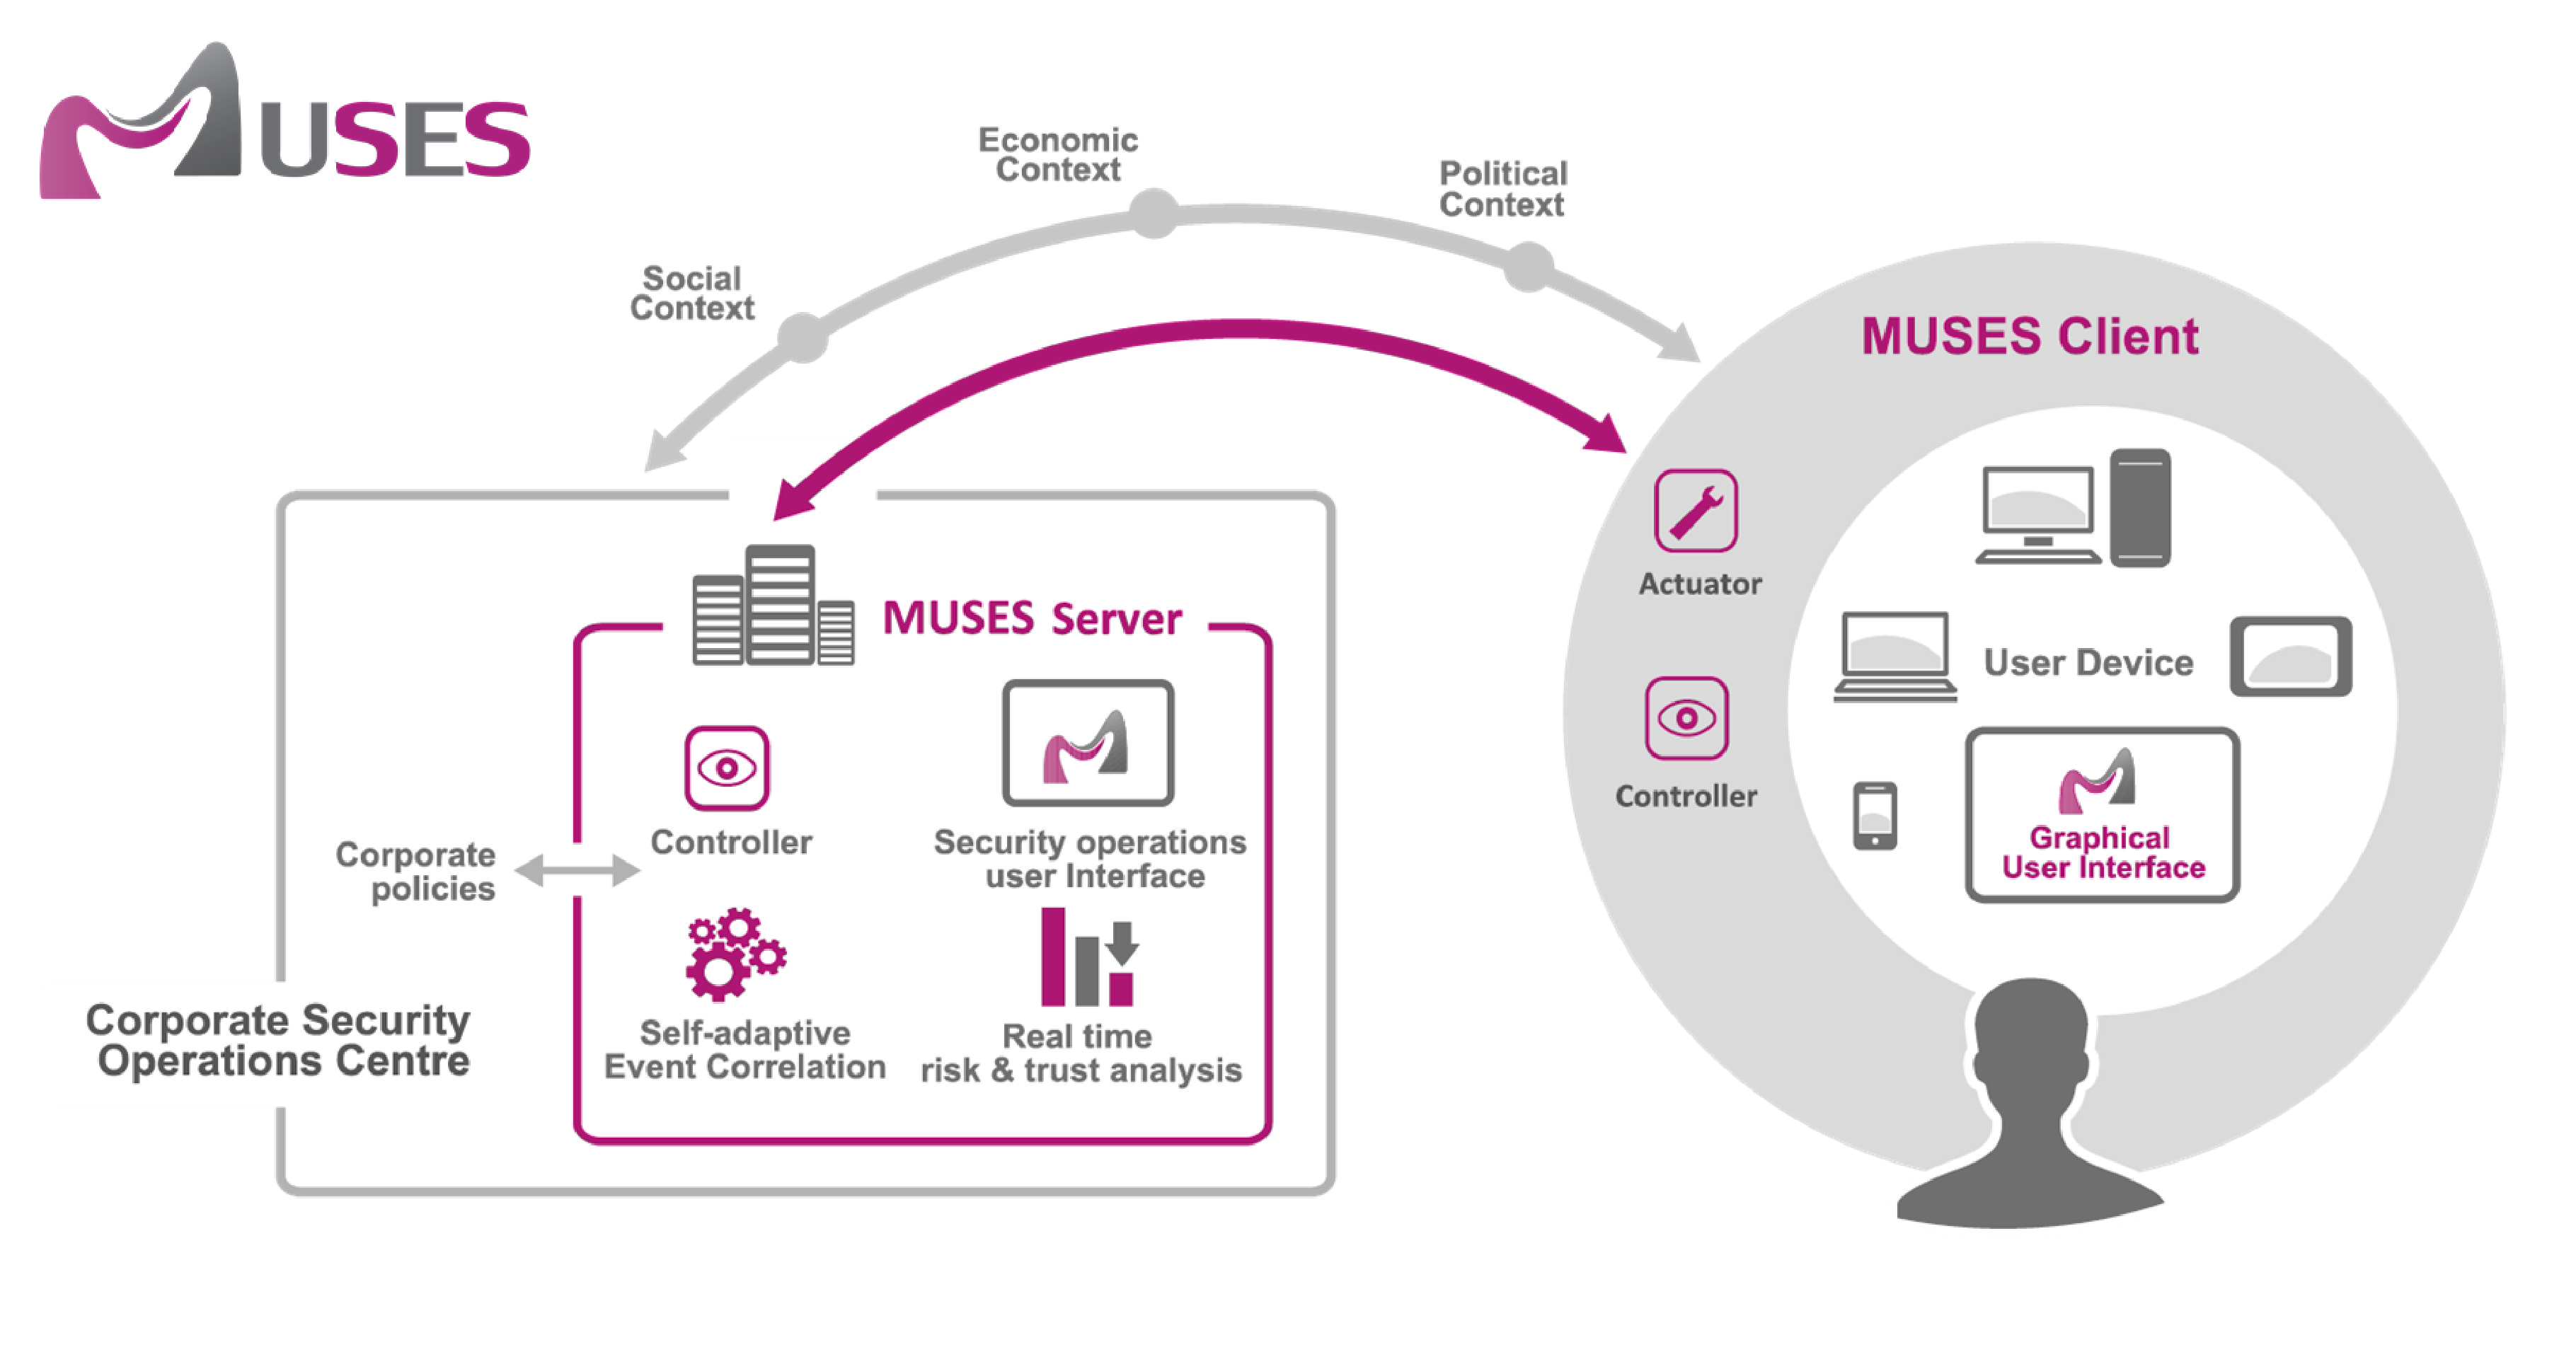
\includegraphics[scale=0.2]{img/system_overview.eps}
\caption{MUSES system overview. Conceptual model designed by S2 Grupo.  http://www.s2grupo.es/.\label{fig:system_overview}}
\end{figure}

As a summary, this application includes two modules: a \textit{controller} and an \textit{actuator}. The first one monitors the environment (context) and the user's behaviour, translating his/her actions into a sequence of events. These events, along with the patterns defining the user's conduct, are processed by the system in real-time by means of a Risk and Trust Analysis Engine (RT2AE) and an Event Correlation module. Then, a decision is taken in the corporate security operations centre (SOC) side, considering the RT2AE output and the set of security rules adapted to that specific user and context. The corresponding feedback is communicated to the user through the \textit{actuator}, which is also in charge of triggering the recommended actions to stop the user's or application's doings, in case it is required.

The designed MUSES architecture is shown in Figure \ref{fig:architecture}. It is a \textit{client/server} approach in which the \textit{client} program will be installed in every user's mobile or portable device, independently of the platform (operating system and type of device). The \textit{server} side would be installed in the corporate SOC. Both sides are connected through a secure channel (using HTTPS) over Internet. In that figure just the high-level components in each part are shown, along with the information flows labelled as 'Info XX'.

\begin{figure}[ht]
%\begin{center}
\hspace{-0.7in}
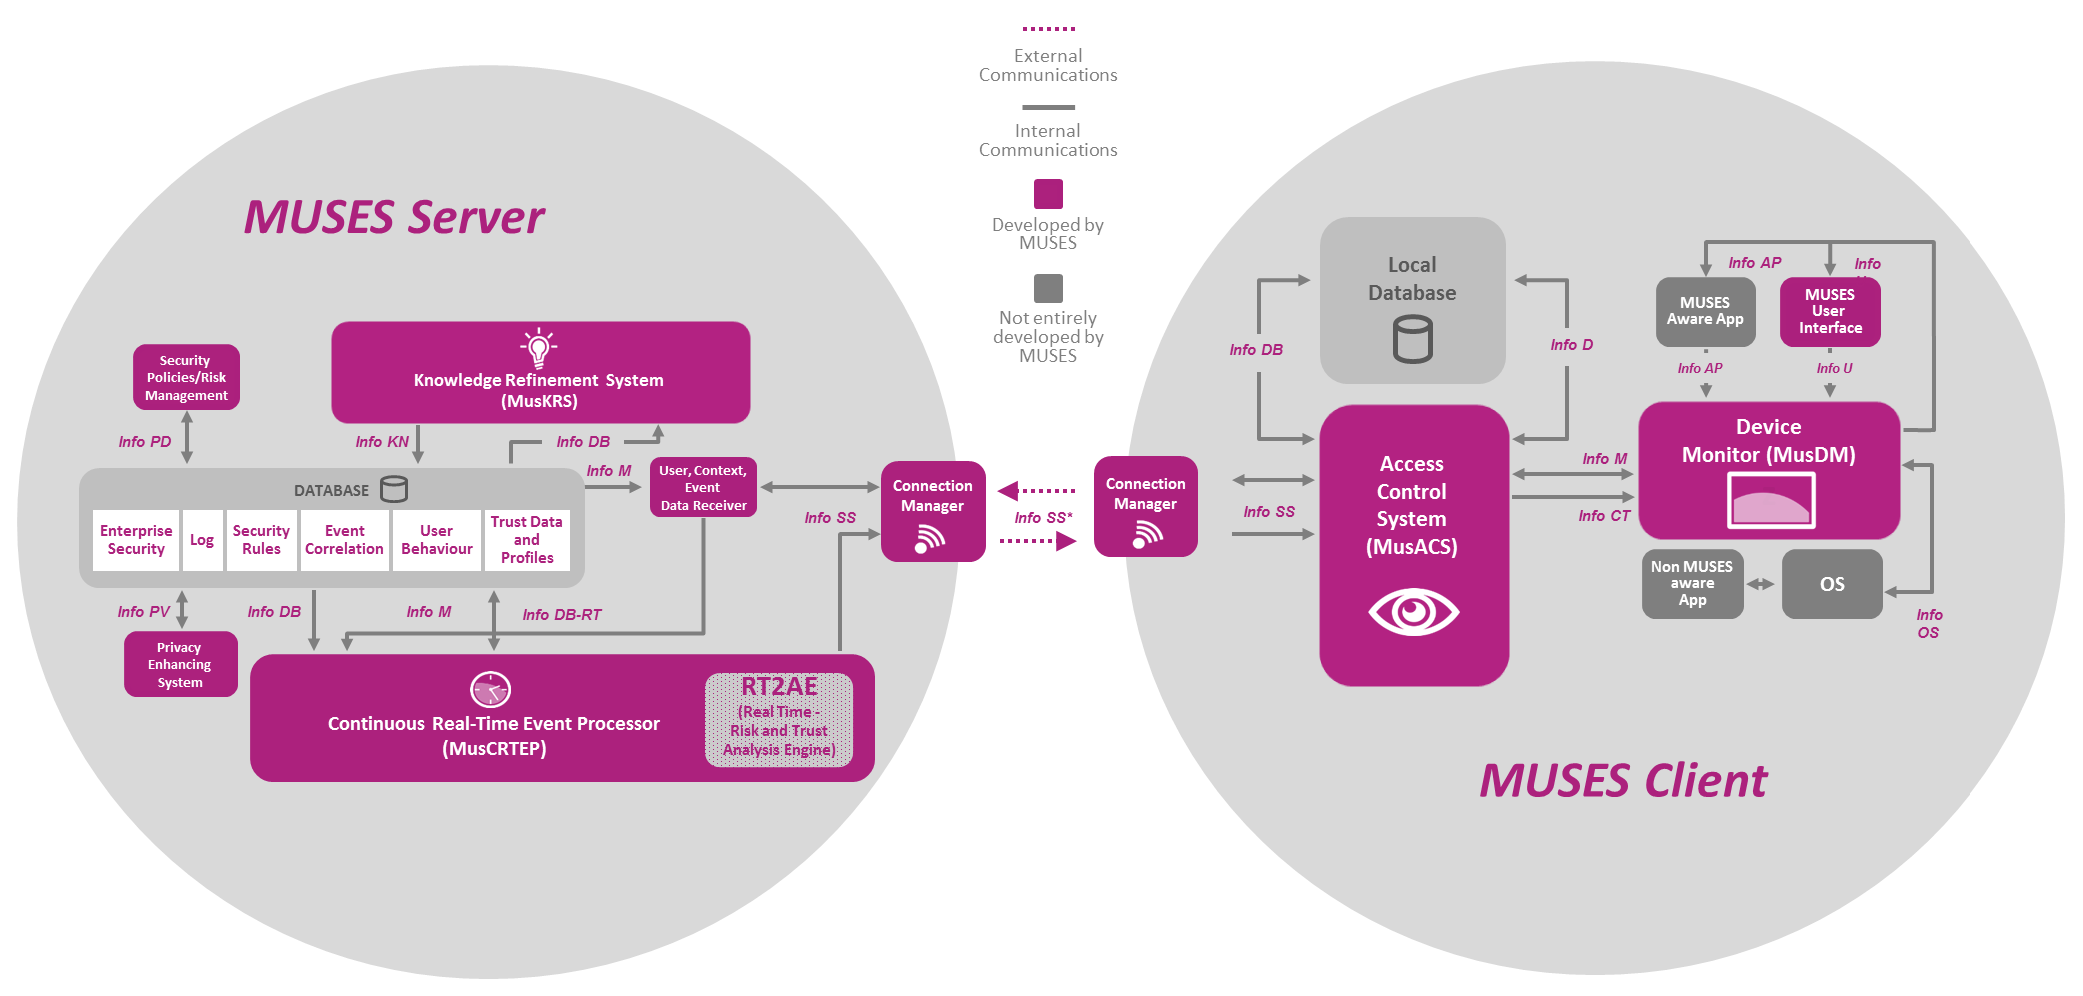
\includegraphics[scale=0.45]{img/architecture_modules.eps}
%\includegraphics[scale=0.45]{img/muses_architecture.eps}
\caption{Design of the MUSES architecture (art by S2 Grupo). \label{fig:architecture}}
%\end{center}
\end{figure}

The rationale for this approach is based on two main reasons: 1) there is need for a high computational power in order to perform the event correlation and self-adaptation processes, so a quite powerful machine should be used (server); 2) there are two clearly separated parts in the system, namely the users (client) and the enterprise (server).

The system considers two working modes for every device: online and offline. In the \textit{online} mode the device can connect with the MUSES server, so it can request the server to make a decision. On the other hand, in \textit{offline} mode the server cannot be reached by the device (there is not an available connection between them), so all the decisions should be made locally.
This will be done using an up-to-date copy on the Decision Table inside the Local database, which will contain decisions for any type of detected event, along with default actions to be performed if no rule is met. Anyway, in this mode, the gathered information by the sensors in the device will be stored for later submission to the server side (when a connection is available), in order to be processed in the knowledge refinement process.
Moreover, when switching from offline to online mode, the device will receive an updated copy of the Decision Rules (the so-called Device Policies), as a kind of antivirus database, in order to work again perfectly in offline mode (if the connection is lost).

All data in MUSES will be encrypted.

% ----------------------------------------------------------

\subsection{Client/Device architecture}

There are three main components in this side:
\begin{itemize}
 	 \item \textit{Local Database}: it is a local security-based storage, which includes the set of security rules to be applied locally (Device Policies), user authentication data, and a cache of gathered events and information. The latter will be useful when the device is in offline mode, so these data are stored to be later submitted to the server side. 
%It contains the so-called \textit{Decision Table}, a set of rules in which the antecedents are high-level events, and the consequents are the corresponding decisions/actions, namely `allow', `deny' or `request' (the decision must be made in the server side).
 	 \item \textit{Device Monitor (MusDM)}: module which gathers the events and information produced by the user. It also acts following the decisions made by the system, in order to allow or deny the controlled application (or the user) for doing something. It is composed by a monitoring and an actuator submodules.
 	 \item \textit{Access Control System (MusACS)}: module in charge of making the decisions considering the gathered data. These decisions can be made locally (if possible), or can be requested to the server (if there is no rule which matches with the occurred events). 

%The subcomponents are the \textit{Decision Maker}, which performs the decision process; the \textit{User, Context, Event Handler}, which processes the events and information to be used for making the decision or stored for further submission (depending on the mode and on the gathered data); and the \textit{Security Policy Receiver} that updates the set of decisions (or Device Policies) in the Decision Table with those received from the server side, after an update or decision process.
\end{itemize}

The rest of the components are: the \textit{MUSES User Interface (UI)}, the application through which the user interacts with the system; and the \textit{Connection Manager} which controls the communications between client and server sides. 
In addition, there are two types of applications considered in this system: on the one hand the \textit{MUSES Aware App}, which is an application adapted to MUSES, so the system can directly interact with it (monitoring and acting). This application must be implemented using the MUSES API (Application Program Interface)\footnote{The MUSES API will be defined in the project, so for every application desired to be MUSES Aware, it should be implemented using this.}. On the other hand the \textit{Non MUSES Aware App} is that which MUSES cannot directly interact with. Usually it will be accessed through the operating system (OS). So the type of information to gather from them and also the type of actions to do over them will vary depending on the OS. In most of the cases MUSES could just detect/recognize very specific events, and also do very limited actions to prevent or block them (maybe showing a screen on the top until something is accomplished by the user). This is due to the usual forbiddance or limitation of interactions with other applications that the OSs have.

% ----------------------------------------------------------

\subsection{Server architecture}

As in the client, there are three main components:
\begin{itemize}
	 \item \textit{System Database}: it stores all the information that the system will manage, including authentication data, enterprise security policies, assets' values, user-related information (trust, context), events data, and, of course, security rules to apply (regarding the security policies).

	 \item \textit{Continuous Real-Time Event Processor (MusCRTEP)}: this component is the core of the MUSES system with respect to the decision making process. It includes an \textit{Event Processor}, the module in charge of performing the event correlation process \cite{EventProcessing_Luckham02,SurveyEventCorrelation_Tiffany02}, gathering the set of occurred events and doing a rule-based threat identification. The output of this module is taken by the \textit{RT2AE}, which also considering information such as trust data and profiles, assets' values, user reputation, or opportunity, performs a risk and trust analysis task \cite{RT2AE_SOTICS13}, and extracts the set of potential rules to consider in the analysed situation. Then, these rules are transformed into decisions (or Device Policies) and submitted to those devices to which they apply.

	 \item \textit{Knowledge Refinement System (MusKRS)}: this module is in charge of analysing the information stored in the system database, identifying relevant data, such as important patterns, key features, or security incidents. These are later processed for tuning up the existing set of rules or for inferring new ones. 

\end{itemize}

There are some other components, namely: the \textit{Security Policies/Risk Management} tool, that lets the company's chief security officer (CSO) to define and manage Security Policies and Rules in a friendly way. It also lets the management of risk-related information, useful for the RT2AE process, such as the assets' values. The \textit{Privacy Enhancing System} which is a module aimed to fit with the legal compliance of the system regarding the user's data anonymisation and retaining of these data in the system. The \textit{User, Context, Event Data Receiver} is devoted to receive data from the device side (events, user-related, etc) and to distribute them among the components (storing in the database, and requesting the Event Processor to start the correlation task). Finally, there is another \textit{Connection Manager} which controls the communication with the device side.


% ----------------------------------------------------------

\subsection{Self-Adaptation in MUSES: The Knowledge Refinement System}

As previously stated, one of the main features of this system will be the self-adaptation (to the user and context), of the set of Corporate Security Rules (specification of the ISPs), that it will be able to perform. 
To this end, the \textit{MusKRS} module will be run asynchronously in the server (once a day or every X hours) and will be in charge of analysing all the gathered information (events, context, user-related data), and adapting/refining the security rules. The refinement (improvement) will have as aim to better deal with these events, optimizing the current set of rules (removing redundant or non-useful rules, for instance), and even trying to predict future threats due to the user's behaviour.

This procedure will be composed by two main steps: first, a Data Mining (DM) \cite{DataMining_Lee01} + Machine Learning (ML) \cite{MachineLearning_Bishop06} process will be performed (in the \textit{Data Miner} sub-component);  second, a refinement and inference process will be done (in the \textit{Knowledge Compiler} sub-component), considering the data `extracted' in the first step, by means of Computational Intelligence (CI) techniques.
It should be noticed that part of the refinement (or adaptation) of the security rules will be made using simpler methods, such as generalisation or specialisation of rules, for instance. Then, other parts of the process would be conducted using CI.

Another important fact is that MUSES will count with a human controller, normally the Chief Security Officer (CSO) of the company, who will supervise the system activity by means of logs or feedback messages. Thus, adapted and inferred security rules will not be, in principle, directly added to the current set of rules. Instead, they will be proposed as draft rules to this controller, in order that he/she will accept them if they are interesting and correct. It is planned that the system will be able to `learn' from this decisions so, after a so-called training or `warm up' period, the rules would be directly accepted (included in the set) or rejected autonomously by the MusKRS.

The following sections describe these processes: first focusing on DM techniques to be used both automatically by the MusKRS, and as a kind of decision-aid/monitoring tool for the CSO; second, the CI techniques are explained, mainly focusing in Evolutionary Computation (EC) \cite{EAs_Back96} approaches, since these methods perform very well, and have been widely used in security-based environments for solving security issues, such as the intrusion detection \cite{GA_intrusion-majeed}, the design and evaluation of security protocols \cite{GP_intrusion-lu,GA_networksecurity-zarza}, or the optimisation of different aspects related with security: IT security costs \cite{EAs_securitycosts-kirta}, and cryptographic protocols \cite{GA_cryptographicprotocols-zarza2}, among others.

% ------------------------------------------------------------------
%
\subsubsection{Data Mining + Machine Learning}
\label{subsubsec:dm_ml}

This task will be performed by the \textit{Data Miner} module. It will take the `raw' data from the database and will process the information, in order to yield a set of relevant data for the Knowledge Compiler module or for the human controller. In the first case, this sub-component will take them as a reference in order to refine or adapt the current set of security rules (for instance, to deal with anomalous situations).

The process will be mainly non-supervised. Moreover, eventually, the datasets can be huge (depending on the company's data flows), so Big Data processing methods \cite{BigData_11} will be applied.

The DM/ML techniques will process the so-called patterns, which in this context correspond to events (and their related information) produced by the users' interactions with the system. As stated, these events will be captured by the sensors in the users' devices and transmitted to the server to be processed and stored in the system database. The methods to be applied are:

\begin{itemize}

\item \textit{Pattern Mining} \cite{PatternMining_Han07}: 
This process will try to identify frequent or, on the contrary, anomalous patterns, in order to process them lately. The idea is that non-frequent patterns are potentially suspicious, and thus, could be of interest to be checked by the CSO or to serve as a reference for the rule-refinement process.

\item \textit{Classification} \cite{classification_67}: 
This technique tries to train a model (classifier) able to associate every pattern in the dataset to a class, so that the model could be used for assign a class for further incoming patterns with an unknown category.
For instance, it could look for events (patterns) that had been previously  marked as `allowed' or `denied' (according to the ISPs). When a new event arises, if it has not an assigned decision, the classifier should provide one based on the similarity with previous (and already labelled) patterns.

\item \textit{Clustering} \cite{Clustering_Jain99}: 
The aim of this method is grouping the patterns considering some similarity criteria, in order to manage them as a set. This could be used for providing data visualisation mechanisms, in order to make it easier to interpret the data interaction and the distribution in clusters with respect to the different properties/features of the patterns.

\item \textit{Feature Selection} \cite{FeatureSelection_Guyon03}: 
It consists on extract the most important features/variables from the data. This could be useful if we want to discard non-key features, which could be interesting in order to reduce the database weight, for improving the performance of other techniques (such as classification or clustering), and even to improve the performance of whole the system, since less information would be gathered and transmitted.

\item \textit{Data Analysis}: 
This will provide the CSO with mechanisms to visualise interesting facts about the data, such as more frequent events, dangerous or suspicious users (according to their behaviour), more triggered rules, etc.

\end{itemize}

%\pagebreak

% ------------------------------------------------------------------
%
\subsubsection{Computational Intelligence: Evolutionary Computation Methods}
\label{subsec:ci}


MUSES will use different EC approaches, initially, two in the DM/ML part of the process, and three in the rule-refinement/adaptation phase. They are based in Genetic Programming (GP) \cite{GP_Koza92}, and Genetic Algorithms (GAs) \cite{GAs_Goldberg89}.

The first evolutionary-based approach will be a \textit{GP-based classification} method. This will be useful for two main reasons: first, in order to deal with the data class imbalance \cite{imbalance_techniques_02}, very common in classification problems inside real systems (with real data); and second, to better manage categorical (non-numeric) data, since most of the features/variables and information gathered from the events take these kind of values.

Thus, this approach will be able to manage unbalanced datasets considering a fitness function in which a cost can be associated to the classifier accuracy at every epoch, having a penalty cost when the classifier makes a false negative (an element from the minority class which is classified as belonging to the majority class) \cite{cost_adjustment_07}.
Regarding the type of data, since GP algorithms can manage rule- or tree-based models, it will work perfectly with any categorical variable, yielding a good classifier as it has been made in other works (such as the aforementioned \cite{cost_adjustment_07}).

The second approach will be a Feature Selection process, conducted using a GA as a meta-algorithm to test all the possible combinations of pattern features/variables in the classification. Thus, the algorithm can optimize the group of features to be considered in the classification task, improving both the computational time of this task and also the obtained accuracy of the method.

The second set of EC techniques are, as stated, part of the rule-refinement (or adaptation) process, to be performed by the \textit{Knowledge Compiler} module. These methods will be used for inference and optimisation, and will consider this data as a part of the process:

\begin{itemize}

\item The information extracted from the Data Miner sub-component, mainly concerning the anomalous, unclassified or misclassified patterns. These are those patterns which did not match with any of the existing classes (they are quite different from the patterns belonging to those classes), so they cannot be included in any of the classes and thus they should be taken into account for a potential inference or update in the set of security rules, in order to `cover' them.

\item User-related information corresponding to those anomalous or unlabelled patterns (events). Thus, the user's ID, location and role, for instance, will be considered in order to select the applicable set of rules for that conditions.

\item Context information for the same patterns, in order to also restrict the applicable set of rules considering this information. 

\end{itemize}

Another useful information to consider in the refinement/ adaptation process will be:

\begin{itemize}

\item Risk information extracted from the user profile (reputation), e.g. "Did the user received a lot of `denies'/`allows' before?", i.e. "Is he/she trustworthy?". In case the user is not, more restrictive rules would be created for him, otherwise the corresponding rules could be `relaxed' for that user.

\item The information stored in logs along the system, which can, for instance, tell about how the user responds to system messages (either an action or if he gives feedback). This could result in the inference of new rules or in adaptation, in order to deal with, for instance, users that repeatedly ignore warning messages.
Moreover, important log information regarding the parameters used or the decisions made in the different modules will be used for further tests of new inferred rules, as it is explained below.

\end{itemize}

Given this, the approaches that will be implemented are:

\begin{itemize}

\item \textit{GP rule inference} method, which will generate/create new rules in order to `cover' those situations non contemplated in the current set of rules. Thus, for instance, a new rule could be created in order to deal with the patterns to which the classifier could not assign a class.
The generation will be done considering the so-called \textit{dictionary}, i.e. a set of terms corresponding to all the possible inputs and actions in the system, which will be antecedents (conditions) and consequents in the security rules to be inferred.
The evaluation of these rules will be done considering the stored log information concerning the parameters along with the actions/decisions made in every component in the system. Thus, it will be possible to `simulate' the whole  system behaviour when the new rule is included and get a value of its performance.

\item \textit{GP rule refinement} approach, which will optimise the current set of rules, adjusting the values in the conditions (antecedents), for instance. Thus, some superfluous parts on the rules and even complete rules could be removed or improved, obtaining for instance specialisations or generalisations of existing rules which could mean a better performance.
The evaluation (of the whole set of security rules) will be done considering the number of unlabelled patterns that will be `covered' after the adjustments.

\item \textit{GA optimisation} algorithm for setting up and adapting the assets' values. These are numerical representations of the importance of the corporate assets, and are considered in the Real-Time Risk and Trust Analysis process, in order to assign a risk value to every potential decision that can be made by the system.
If it is possible to evaluate the partial solutions proposed by the GA, this approach could be very useful for the CSO (who is in charge of assigning and adjusting these values over time).
The adaptation or adjustment concerns the change in value that an asset could have due to a loss of importance, once an event has passed (a project presentation, for instance).

\end{itemize}


%----------------------------------------------------------------------------
%%%%%%%%%%%%%%%%%%%%%%%%%%%%%%%   COMPARISON  %%%%%%%%%%%%%%%%%%%%%%%%%%%%%%%
%----------------------------------------------------------------------------

\section{MUSES Advantages over Other Solutions. Beyond the State of the Art}
\label{sec:comparison}


MUSES is mainly a free, open-source, platform independent solution, so these set of features make it a very good option in a first comparison against most of the proprietary, close and system-specific tools presented in Section \ref{sec:toolsreview} (all but WSO2). In addition most of the existing tools take into account only smartphones and tablets, but MUSES also will cover laptops and company PCs too, thus, it is not only for BYOD. Moreover the companies which desire work with those systems need specific operative system and server (such as Windows Server, for instance), being even more strict in some cases, as in Samsung Knox, in which companies must work with a specific (though they can choose from a list) MDM service for being able of deploy Knox in their environments, or in the use of the Blackphone. MUSES will be a good solution in these cases, since it will be a multiplatform system. 

Another comparison concerns that the existing products are mostly policy-based, but MUSES makes its decisions not only considering policies, but also based on the terminals/users context (location, connected networks and so on), to really understand the real danger of a specific action, i.e. it adds a Risk Analysis Process (performed in the RT2AE).

Also related to this issue, a very big plus of the MUSES system (not present in the other solutions) is its self-adaptivity power. Thus, MUSES is able to adapt to changes, either regarding corporate security policies, newly discovered vulnerabilities or threats, different environments of use, or user profiles. 

Moreover, another clear advantage over the rest is that MUSES can work in two connection modes, depending on the client being able to connect with the server or not, which favours a real-time decision making process.

Though these are clearly advantages of MUSES over the aforementioned products, they also establish a progress beyond the state of the art with respect to the existing solutions. Other issues that MUSES aims to progress on are related to risk and trust data analysis, human-computer interaction (or HCI), device monitoring, and legal compliance. 

First, as mentioned previously, it will implement a self-adaptive event correlation, including a novel hybrid technique of rule refinement and rule adjustment extracting relevant information from processing huge amounts of data. Then, the project defines a new approach to risk management taking into account threats (with their costs) as well as the innovative concept of opportunity, i.e. the following beneficial outcome from a situation on which, for instance, a user is able to work while waiting at the airport if risk is low enough. 

About HCI and usability of mobile devices, this will set up a significant advance in the state of the art because of the novelty of the BYOD philosophy, and trying to look for individual differences among the users in susceptibility to persuasive strategies for secure behaviour. Regarding device monitoring, MUSES will also take into account the so-called context observation, by which private or professional scenarios will be detected, or predicted, based on advanced machine learning techniques. Finally, the project is concerned about legal compliance in regards of Information Security Policies, so that it will contribute to the proposal for the EU Data Protection: legal binding force and legal certainty of company policies, and end-user responsibility.

With regard to the scientific contribution of the system, one of the main differences with respect to previous works is the consideration of security threats `brought' by the user's behaviour inside the system, i.e. through interaction/events, rather than more general and external threats. Moreover, the techniques to be used in MUSES will work with real data (in a real system), as a difference to several research works (they consider simulated or artificial data).

Data Mining techniques have been used by the authors in some works, but usually aiming for a specific general objective, for instance the detection of threats (botnet) \cite{botnet_detection_clustering_09}, or the recognition of anomalies \cite{feature_selection_anomalies_08}, but they are not linked with a following process to improve the system (the refinement phase in MUSES).

There are some proposals in which security policies are inferred or refined \cite{inferring_policies_socialnetworks_09,policy_generation_clustering_10}, but they do not affect the ISPs as in MUSES, and they are not based in the user's behaviour in order to do this.

Genetic Programming has been previously used by several authors \cite{rule_generation_gp_09,sec_policy_evolution_gp_08}, even for creating new policies or rules in a security-aimed sense, but they do not affect the ISPs and moreover, our proposed evaluation functions (completely integrated in the system) for the refinement and inference approaches are novel.

With respect to Genetic Algorithms, they have been extensively used in this scope in the literature, mainly for the detection of anomalies and intrusions rather than for optimisation, as in our case. However, there are some examples that could be used as model for our approach, such as \cite{EAs_securitycosts-kirta,risk_reduction_ga_12}.

	
%*** Features:
%Concept of framework-enabled app (Citrix' Worx-enabled apps == MUSES-aware app)
%
%*** Azzurri includes several of the MUSES features


%----------------------------------------------------------------------------
%%%%%%%%%%%%%%%%%%%%%%%%%%%%%%%   CONCLUSIONS  %%%%%%%%%%%%%%%%%%%%%%%%%%%%%%%
%----------------------------------------------------------------------------

\section{Conclusions}
\label{sec:conclusions}

In this work, there is introduced a self-adaptive user-centric end-to-end system, named MUSES, which is in development (it will be launched next year). The architecture and main features of the system are described, paying special attention to the application of Soft Computing methods in tasks of data analysis, machine learning, and also in the use of evolutionary algorithms to improve the existing set of corporate security rules which leads the system.

MUSES has been compared with other existing solutions/tools with a similar aim: to ensure the protection and privacy of sensitive information in the enterprise when it is accessed by the employees using their own devices (BYOD philosophy).
The main advantages of MUSES with respect to the other solutions have been discussed, also remarking its advances beyond the state of the art that define these tools.

In addition, a scientific comparison between the techniques used in the presented system and those in the literature, in the same scope, has been done.

We can conclude that MUSES offers several advantages over the existing tools, both the some of its `technical' features, but also in the application of Data Mining, Machine Learning and Computational Intelligence methods to the events gathered by the system (users' behaviour), in order to adapt or refine the set of security rules.

Anyway, there is room for considering some of the existing researches that could be added as future features for MUSES, such as the analysis of users via social networks \cite{inferring_policies_socialnetworks_09,user_classification_ml_13}, the optimisation of security protocols \cite{GA_networksecurity-zarza}, the implementation of intrusion detection mechanisms \cite{GA_intrusion-majeed}, or the application of novel privacy-related techniques \cite{AAI_book_2009}, which is another feature also considered in MUSES.

%%%%%%%%%%%%%%%%%%%%%%%%%%%%%  ACKNOWLEDGEMENTS %%%%%%%%%%%%%%%%%%%%%%%%%%%%%%%%

\section{Acknowledgements}
This paper has been funded in part by European project MUSES
(FP7-318508), along with Spanish National projects
TIN2011-28627-C04-02
(ANYSELF) and TIN2014-56494-C4-3-P (EphemeCH), and GENIL PYR-2014-17,
awarded by the CEI-BioTIC UGR.  

\bibliographystyle{elsarticle-num}
\bibliography{geneura-latin1,review_muses}

% Antonio - Poner la bibliograf�a en fichero .bib

%\begin{thebibliography}{00}

%\bibitem{ids13}
%Sommestad T., Hunstad A.. \emph{Intrusion detection and the role of the system administrator.}, from Swedish Defence Research Agency (FOI), Link�ping, Sweden, 2013.

%\bibitem{m2m12}
%NTT DOCOMO, \emph{DOCOMO to Launch Global M2M Platform}, in M2M Magazine, December 2012.
%http://www.machinetomachinemagazine.com/2012/12/05/docomo-to-launch-global-m2m-platform/.

%\bibitem{suites12}
%The Radicati Group Inc., report \emph{Microsoft Office 365 - Analysis and Forecast, 2012-2016}. June 2012. 

%\bibitem{Adams_Users05}
%Adams, A. and Sasse, A.:
%\newblock {\em Users are not the enemy}.
%\newblock Security and Usability: Designing Systems That People Can Use.
%  O\'Reilly Associations, 2005.

%\bibitem{cost_adjustment_07}
%Alfaro-Cid, E., Sharman, K. and Esparcia-Alc�zar, A.I.:
%\newblock A genetic programming approach for bankruptcy prediction using a
%  highly unbalanced database.
%\newblock In M.~Giacobini, editor, {\em Applications of Evolutionary
%  Computing}, volume 4448 of {\em Lecture Notes in Computer Science}, pages
%  169--178. Springer Berlin Heidelberg, 2007.

%\bibitem{AzurriMDM}
%Azurri Communications.
%\newblock Icon Mobilise.
%\newblock \url{http://www.azzurricommunications.com/~/media/Resources/Brochures/Media/icon_mobilise_brochure_online.ashx}

%\bibitem{SecPolComp12}
%Al-Omari, A., El-Gayar, O., Deokar, A., and Walters, J.: \emph{Security Policy Compliance: User Acceptance Perspective}. 45th Hawaii International
%Conference on System Sciences (pp. 3317-3326). IEEE, 2012.

%\bibitem{BYOD13}
%Bacik, S.: \emph{Security Implications of Bring Your Own Device, IT Consumerization, and Managing User Choices}, in Information Security Management Handbook, Sixth Edition, Volume 7, pp. 133-142, 2013.

%\bibitem{EAs_Back96}
%Back, T.:
%\newblock {\em Evolutionary algorithms in theory and practice}.
%\newblock Oxford University Press, 1996.

%\bibitem{MachineLearning_Bishop06}
%Bishop, C.:
%\newblock {\em Pattern recognition and Machine Learning}.
%\newblock Springer, 2006.

%\bibitem{Blackberry_tool}
%Blackberry.
%\newblock Blackberry balance.
%\newblock \url{http://es.blackberry.com/business/software/blackberry-balance.html}

%\bibitem{Blackphone}
%Blackphone.
%\newblock \url{https://www.blackphone.ch/}


%\bibitem{SecPolComp10}
%Bulgurcu, B., Cavusoglu, H., and Benbasat, I.: \emph{Information security policy compliance: an empirical study of rationality-based beliefs and information security awareness}. MIS Quarterly, 34(3), 523-548. 2010.

%\bibitem{botnet_detection_clustering_09}
%Chang, S. and Daniels, T.E.:
%\newblock P2P botnet detection using behavior clustering \& statistical tests.
%\newblock In {\em Proceedings of the 2nd ACM Workshop on Security and
%  Artificial Intelligence}, AISec '09, pages 23--30, New York, NY, USA, 2009.
%  ACM.

%\bibitem{SecPol09}
%Cresson Wood, C. and Lineman, D.: \emph{Information Security Policies Made Easy Version 11}. Information Shield, Inc. 2009.

%\bibitem{inferring_policies_socialnetworks_09}
%Danezis, G.:
%\newblock Inferring privacy policies for social networking services.
%\newblock In {\em Proceedings of the 2Nd ACM Workshop on Security and
%  Artificial Intelligence}, AISec '09, pages 5--10, New York, NY, USA, 2009.
%  ACM.

%\bibitem{Good_tool}
%Good's Technology.
%\newblock BYOD Solution.
%\newblock
%  \url{http://www1.good.com/secure-mobility-solution/bring-your-own-device.html}

%\bibitem{GAs_Goldberg89}
%Goldberg, D.E.:
%\newblock {\em Genetic Algorithms in search, optimization and machine
%  learning}.
%\newblock Addison Wesley, 1989.

%\bibitem{FeatureSelection_Guyon03}
%Guyon, I.,  and Elisseeff, A.:
%\newblock An introduction to variable and feature selection.
%\newblock {\em J. Mach. Learn. Res.}, 3:1157--1182, 2003.

%\bibitem{PatternMining_Han07}
%Han, J., Cheng, H., Xin, D., and Yan, X.:
%\newblock Frequent pattern mining: Current status and future directions.
%\newblock {\em Data Min. Knowl. Discov.}, 15(1):55--86, 2007.

%\bibitem{SecPolPenalty09}
%Herath, T., and Rao, H.R.: \emph{Protection motivation and deterrence: a framework for security policy compliance in organisations}. European Journal of Information Systems, vol. 18, pp. 106-125, 2009.
	
%\bibitem{IBM_tool}
%IBM.
%\newblock Hosted mobile device security management.
%\newblock
%\url{http://www-935.ibm.com/services/us/en/it-services/managed-security-services-cloud-computing} \url{ -hosted-mobile-device-security-management.html}

%\bibitem{Clustering_Jain99}
%Jain, A.K., Murty, M.N., and Flynn, P.~J.:
%\newblock Data clustering: A review.
%\newblock {\em ACM Comput. Surv.}, 31(3):264--323, Sept. 1999.

%\bibitem{imbalance_techniques_02}
%Japkowicz, N. and Stephen, S.:
%\newblock The class imbalance problem: A systematic study.
%\newblock {\em Intell. Data Anal.}, 6(5):429--449, Oct. 2002.

%\bibitem{ibm11}
%Kao, I-L.: \emph{IBM Security Services. Securing mobile devices in the business environment}, IBM, 2011.

%\bibitem{feature_selection_anomalies_08}
%Kloft, M., Brefeld, U., D\"{u}essel, P., Gehl, C. and Laskov, P.:
%\newblock Automatic feature selection for anomaly detection.
%\newblock In {\em Proceedings of the 1st ACM Workshop on Workshop on AISec},
%  AISec '08, pages 71--76, New York, NY, USA, 2008. ACM.

%\bibitem{GP_Koza92}
%Koza, J.~R.:
%\newblock {\em Genetic Programming: On the programming of computers by means of
%  natural selection}.
%\newblock MIT Press, Cambridge, MA, 1992.

%\bibitem{EAs_securitycosts-kirta} 
%Kirta, T., and Kivimaab, J.: Optimizing it security costs by evolutionary algorithms. In C. Czosseck and K. Podins, editors, Conference on Cyber Con ict,pages 145-160, CCD COE Publications, 2010.

%\bibitem{DataMining_Lee01}
%Lee, S.J. and Siau, K.:
%\newblock A review of data mining techniques.
%\newblock {\em Industrial Management \& Data Systems}, 101(1):41--46, 2001.

%\bibitem{user_classification_ml_13}
%Leontjeva, A., Goldszmidt, M., Xie, Y., Yu, F. and Abadi, M.:
%\newblock Early security classification of skype users via machine learning.
%\newblock In {\em Proceedings of the 2013 ACM Workshop on Artificial
%  Intelligence and Security}, AISec '13, pages 35--44, New York, NY, USA, 2013.
%  ACM.

%\bibitem{sec_policy_evolution_gp_08}
%Lim, Y.T., Cheng, P.C., Rohatgi, P. and Clark, J.A.:
%\newblock Mls security policy evolution with genetic programming.
%\newblock In {\em Proceedings of the 10th Annual Conference on Genetic and
%  Evolutionary Computation}, GECCO '08, pages 1571--1578, New York, NY, USA,
%  2008. ACM.

%\bibitem{MIT05}
%Lippmann, R.P., Ingols, K.W., Scott, C., Piwowarski, K., Kratkiewicz, K.J., Artz, M., and Cunningham, R.K.: \emph{Evaluating and Strengthening Enterprise
%Network Security Using Attack Graphs}. Project Report IA-2. Lincoln Laboratory, Massachusetts Institute of Technology, October 2005.

%\bibitem{GP_intrusion-lu} Lu, W. and Traore, L.: Detecting new forms of network intrusion using genetic programming. In Proceedings of the 2003 Congress on Evolutionary Computation, pages 2165-2172, 2003.

%\bibitem{EventProcessing_Luckham02}
%Luckham, D.:
%\newblock {\em The Power of Events: An Introduction to Complex Event Processing
%  in Distributed Enterprise Systems}.
%\newblock Addison-Wesley, MA, USA, 2002.

%\bibitem{classification_67}
%MacQueen, J.:
%\newblock Some methods for classification and analysis of multivariate
%  observations.
%\newblock In {\em Proceedings of the fifth Berkeley symposium on mathematical
%  statistics and probability}, volume~1, page~14. California, USA, 1967.

%\bibitem{GA_intrusion-majeed} Majeed, P.G. and Kumar, S. Genetic algorithms in intrusion detection systems: A survey. International Journal of Innovation and Applied Studies, 5(3):233-240, March 2014.

%\bibitem{Opp_Security11}
%Oppliger, R.:
%\newblock Security and privacy in an online world.
%\newblock {\em IEEE Computer}, 44(9):21--22, September 2011.

%\bibitem{android11}
%Orthacker, C., Teufl, P., Kraxberger, S., Lackner, G., Gissing, M., Marsalek, A., Leibetseder, J., and Prevenhueber, O.: \emph{Android Security Permissions - Can We Trust Them?}. MobiSec Session on Smartphone Security, Aalborg 2011.

%\bibitem{BigData_11}
%Ratner, B.:
%\newblock {\em Statistical and Machine-Learning Data Mining: Techniques for
%  Better Predictive Modeling and Analysis of Big Data, Second Edition}.
%\newblock CRC Press, Inc., Boca Raton, FL, USA, 2nd edition, 2011.

%\bibitem{policy_generation_clustering_10}
%Samak, T. and Al-Shaer, E.:
%\newblock Synthetic security policy generation via network traffic clustering.
%\newblock In {\em Proceedings of the 3rd ACM Workshop on Artificial
%  Intelligence and Security}, AISec '10, pages 45--53, New York, NY, USA, 2010.
%  ACM.

%\bibitem{Samsung_tool}
%Samsung KNOX.
%\newblock
%  \url{https://www.samsungknox.com}

%\bibitem{Schu_SecPatterns05}
%Schumacher, M., Fernandez-Buglioni, E., Hybertson, D., Buschmann, F., and
%  Sommerlad, P.:
%\newblock {\em Security Patterns: Integrating Security and Systems
%  Engineering}.
%\newblock John Wiley \& sons, 2005.

%\bibitem{RT2AE_SOTICS13}
%Seigneur, J.-M., K�lndorfer, P., Busch, M., and Hochleitner, C.:
%\newblock A survey of trust and risk metrics for a BYOD mobile working world.
%\newblock In {\em Third International Conference on Social Eco-Informatics
%  (SOTICS 2013)}, page To Appear. Curran Associates Inc., November 2013.

%\bibitem{SecPolComp09}
%Shaw, R.S., Chen, C.C., Harris, A.L., and Huang, H.-J.: \emph{The impact of information richness on information security 
%awareness training effectiveness}. Computers \& Education, vol. 52, pp. 92-100, 2009.

%\bibitem{SecPolComp07}
%Siponen, M., Pahnila, S., and Mahmood, A.: \emph{Employees' adherence to information security policies: an empirical study}. In IFIP International Federation for Information Processing, Volume 232, New Approaches for Security, Privacy and Trust in Complex Environments pp. 133-144, 2007.

%\bibitem{AAI_book_2009}
%Solanas, A. and Mart�nez-bal, A.:
%\newblock {\em Advances in Artificial Intelligence for Privacy Protection and
%  Security}.
%\newblock World Scientific Publishing Co., Inc., River Edge, NJ, USA, 2009.

%\bibitem{Sophos_tool}
%Sophos.
%\newblock Mobile control.
%\newblock \url{http://www.sophos.com/en-us/products/mobile-control.aspx}
%
%\bibitem{rule_generation_gp_09}
%Suarez-Tangil, G., Palomar, E. Fuentes, J., Blasco, J. and Ribagorda, A.:
%\newblock Automatic rule generation based on genetic programming for event
%  correlation.
%\newblock In l.~Herrero, P.~Gastaldo, R.~Zunino, and E.~Corchado, editors, {\em
%  Computational Intelligence in Security for Information Systems}, volume~63 of
%  {\em Advances in Intelligent and Soft Computing}, pages 127--134. Springer
%  Berlin Heidelberg, 2009.

%\bibitem{risk_reduction_ga_12}
%Tamjidyamcholo, A.:
%\newblock Genetic algorithm approach for risk reduction of information
%  security.
%\newblock {\em International Journal of Cyber-Security and Digital Forensics
%  (IJCSDF)}, 1(1), 2012.

%\bibitem{SurveyEventCorrelation_Tiffany02}
%Tiffany, M.:
%\newblock A survey of event correlation techniques and related topics.
%\newblock Research paper, Georgia Institute of Technology, 2002.

%\bibitem{WorxSDK}
%Citrix.
%\newblock Worx App SDK.
%\newblock \url{http://www.citrix.es/go/worx-app-sdk.html}
%
%\bibitem{WSO2_tool}
%WSO2.
%\newblock Enterprise Mobility Manager.
%\newblock \url{http://wso2.com/products/enterprise-mobility-manager/}

%\bibitem{GA_networksecurity-zarza} 
%Zarza, L., Forn�, J., Pegueroles, J.R., and Soriano, M.: Advances in artificial intelligence for privacy protection and security, chapter Genetic algorithms for designing network security protocols, pages 325-358. World Scientific, 2010.
%
%\bibitem{GA_cryptographicprotocols-zarza2} 
%Zarza, L., Pegueroles, J., Soriano, M., and Mart�nez, R.: Design of cryptographic protocols by means of genetic algorithms techniques. In M. Malek, E. Fern�ndez-Medina, and J. Hernando, editors, SECRYPT, pages 316-319. INSTICC Press, 2006.

%\end{thebibliography}


\end{document}
%%% Local Variables:
%%% ispell-local-dictionary: "english"
%%% hunspell-local-dictionary: "english"
%%% End:
